% !TEX root = diplomarbeit.tex
\chapter{Bilder}
\label{bilder}
\thispagestyle{empty}

Wie binde ich eigentlich ein Bild ein ?

\begin{figure}[ht]
 \centering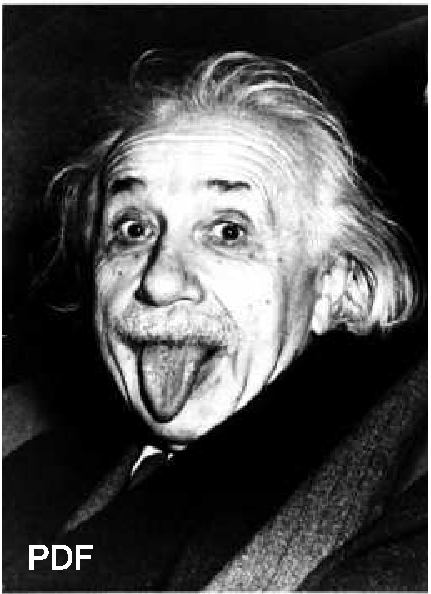
\includegraphics[width=0.6\textwidth]{einsteinlabel.pdf}
 \caption[Einstein-pdf]{Toller Typ. Das hier ist ein PDF (Vektorgrafik-f"ahiges Format).}
 \label{piceinsteinpdf}
\end{figure}

\begin{figure}[ht]
 \centering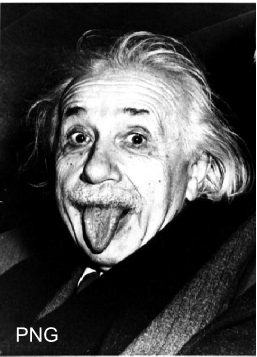
\includegraphics[width=0.6\textwidth]{einsteinlabel.png}
 \caption[Einstein-png]{Toller Typ. Das hier ist ein PNG (Bitmap-Format).}
 \label{piceinsteinpng}
\end{figure}

Wie binde ich ein Bild ein, das ich mit Matlabfrag erzeugt habe? (F�r eine genauere Erl�uterung zu Matlabfrag and Gnuplot schau Dir die Plauderstunde im Wiki zu diesem Thema an.)

\begin{figure}[ht]
 \centering
 \psfragfig[width=0.7\textwidth]{pics/APsMfrag}
 \caption[Aktionspotential]{Grafik erzeugt mit Psfrag (der Text in der Grafik wird durch die aktuelle LateX-Schriftart in der passenden Schriftgr��e ersetzt}
 \label{piceinsteinpng}
\end{figure}
